\documentclass{article}

\usepackage[margin=1in]{geometry}
\usepackage[T1]{fontenc}
\usepackage{amsmath}
\usepackage{booktabs}
\usepackage{tabularx}
\usepackage{enumitem}
\usepackage{xcolor}
\usepackage{tikz}
\usetikzlibrary{arrows.meta,positioning}
\usepackage[hidelinks]{hyperref}

\definecolor{cablue}{RGB}{31,78,121}
\definecolor{cagrey}{RGB}{95,95,95}
\definecolor{calight}{RGB}{233,239,245}
\definecolor{caamber}{RGB}{176,110,20}
\definecolor{cared}{RGB}{155,40,40}
\definecolor{cagreen}{RGB}{40,105,65}

\newcommand{\vd}[1]{\texttt{\detokenize{#1}}}

\setlist{nosep,leftmargin=1.3em}

\title{CiteAudit: Automated Bibliographic Auditing for Validating Citation Existence, Retraction Status, and Claim Alignment in Academic Manuscripts}

\author{%
Hussein Nasereddine\textsuperscript{1}, Walid Chaar\textsuperscript{2}, and Ali Kalakech\textsuperscript{3}\\[6pt]
\small\textsuperscript{1}Independent Research Engineer, Beirut, Lebanon\\
\small\textsuperscript{2}Research Department, Novum Research, Beirut, Lebanon\\
\small\textsuperscript{3}Engineering Department, Lebanese International University, Beirut, Lebanon\\
\small Corresponding author: \href{mailto:husseinnaserddine21@gmail.com}{husseinnaserddine21@gmail.com}%
}
\date{Version 1.2, September 2026}

\begin{document}

\maketitle

\begin{abstract}
Checking citations by hand is slow, and it often misses retracted papers, references that do not exist, and claims that the cited source does not support. This paper presents CiteAudit, a web tool that checks the references of an uploaded manuscript. It finds the in-text citations and the part of the sentence each one supports, looks up every reference in up to six scholarly indexes (Crossref, OpenAlex, Semantic Scholar, arXiv, Europe PMC, and Unpaywall), checks for retractions, and judges whether each cited source supports its claim, using a word-overlap method and an optional language model. For every reference it also saves visual evidence: the citing sentence, the header of the source, and the matching passage, or an abstract card when the full text cannot be reached. We describe the design, give the exact existence score and its thresholds, list the language-model settings, and check each description against the source code. The offline test suite has 192 tests, all passing, and runs in about 7 seconds. On four published manuscripts (117 pages, 364 references, 444 judged claims), the tool took 3.5 to 5.3 seconds per reference. It confirmed 329 references (90.4\%), left 15 (4.1\%) for a person to check, and found no index match for 20 (5.5\%). Full text was found for only 13.4\% of the references we analysed for coverage; 58.9\% were judged on their abstract alone. A benchmark with up to ten manuscripts running at once finished every run, but rate limits cut the share of references judged by the model from 100\% to 79.3\%, and the benchmark revealed a bug in how throttled index replies were handled, which we fixed. These results describe speed, outcomes, and coverage. They do not measure accuracy, which needs a labelled dataset that we have not yet built.
\end{abstract}

\section{Introduction}
\label{sec:intro}

Citations link new research to earlier work, so the scientific record depends on them being correct. Checking a bibliography by hand takes time and can miss broken references, retracted papers, wrong author names, and claims that the source does not support \cite{ref1}. The problem is well known. A meta-analysis found quotation errors in about one in four citations in medical journals \cite{jergas2015,mogull2017}, and similar rates have been reported in general science journals \cite{smith2020} and in older studies \cite{delacey1985,evans1990}. Citations that misstate their sources, or that keep citing retracted work \cite{hsiao2021,schneider2020}, weaken the record.

Today, this checking is done by authors, reviewers, and copy editors, which is slow and hard to scale \cite{ref1,aczel2021}. Existing automated tools often rely on scattered data sources or strict title matching, or they judge a group of citations as one unit, which can hide a single unsupported claim. They also struggle with paywalled content and with telling an index that is down apart from a work that does not exist \cite{ref1,ref9,ref10}. CiteAudit aims to make citation screening more consistent and easier to check \cite{ref4}. It combines reference checking across several indexes \cite{ref1}, checking of each claim \cite{ref2,ref8}, and automatic evidence capture \cite{ref3}, and it summarises the results in a short risk report \cite{hicks2015}.

\subsection{Background and Motivation}

The volume of scientific literature keeps growing \cite{bornmann2015}, and generative AI is now widely used in writing. AI has raised the risk of unsupported claims, invented citations, and mismatched citations \cite{walters2023,bhattacharyya2023,ji2023}, on top of existing concerns about the reliability of published research \cite{baker2016}. Manual checking cannot keep up with this volume. An automated check can help, but only if its results are transparent and easy for a person to verify. This is the problem we address.

\subsection{Problem Statement}

Generative AI has changed how academic text is produced \cite{ref5,ref6}. Large language models can draft manuscripts quickly, but they can also add serious errors to the research record \cite{ref10}. One of the main errors is citation hallucination: references that look real but do not exist \cite{ref3,alkaissi2023,day2023}. Early studies found that many generated references were fabricated \cite{walters2023}, and that about half of the references in some AI-generated medical texts did not exist \cite{bhattacharyya2023}. The problem persists in newer systems, with hallucination rates between $14.2\%$ and $94.9\%$ across thirteen models and 375{,}440 generated citations \cite{ref9}. Another study found that no model reached a citation-level existence rate above $0.475$ under controlled prompts \cite{ref10}. This follows from how these models generate text, so it is not a simple bug that can be patched \cite{ji2023}. Even when a cited source exists, an AI system may cite it for a claim it does not support \cite{ref8}.

Traditional checking has its own limits. It relies on manual inspection or simple title matching, and it usually treats each reference as one block instead of checking each claim \cite{ref1,ref2}. It also does not scale to large numbers of submissions \cite{aczel2021}, so reviewers find it hard to catch citation errors and retracted papers \cite{ref4}. More than ten thousand papers were retracted in 2023 \cite{vannoorden2023,brainard2018}, many of them linked to large-scale fraudulent publishing \cite{else2021,cabanac2021prev,byrne2017}. Retractions are also easy to miss, and retracted papers continue to be cited for years, often without any mention of the retraction \cite{hsiao2021,barilan2017,wager2011}.

These errors can pass peer review. An audit of 2.5 million biomedical papers with 125.6 million references found 4{,}046 fabricated references in 2{,}810 papers, a twelve-fold increase between 2023 and early 2026, reaching about one paper in 277 \cite{ref5}. Another study found that about one in twenty accepted papers at top machine learning and security venues had at least two likely hallucinated references \cite{ref6}. What is needed is an automated, scalable tool that checks both whether each reference is real and whether it supports the claim it is cited for.

\subsection{Existing Solutions}
\label{sec:related}

Among retrieval-based systems, \textbf{BibAgent} \cite{ref1} combines several indexes and aggregates evidence to detect miscitations. When full text is behind a paywall, it uses agreement between later citing papers instead. It was evaluated with a five-category miscitation taxonomy and a benchmark of 6{,}350 samples across 254 fields. \textbf{GhostCite} provides \textsc{CiteVerifier}, a multi-source retrieval and similarity-matching pipeline that it applied to 2.2 million citations \cite{ref9}. For checking whether a source supports a claim, \textbf{SemanticCite} \cite{ref2} analyses the full text and uses four classes: Supported, Partially Supported, Unsupported, and Uncertain. \textbf{DeepTRACE} \cite{ref8} audits AI research assistants by breaking their answers into citation matrices and testing whether each reference supports each statement.

Other lightweight tools check references offline on ordinary hardware \cite{ref3}. Some auditing protocols check every reference against several databases without assuming it is valid; one such study verified $91.7\%$ of 2{,}581 references with a false-positive rate below $0.5\%$ \cite{ref4}. These tools sit alongside large audits of biomedical \cite{ref5} and technical \cite{ref6} literature and studies of how prompting affects citation accuracy \cite{ref10}.

Three related areas also inform this work. First, automated integrity screening already exists for other problems. For example, \texttt{statcheck} recomputes reported statistics and flags inconsistencies \cite{nuijten2016,nuijten2020}, the Rigor and Transparency Index rates how well methods are reported \cite{menke2020}, and other tools flag problematic preprints \cite{weissgerber2021} and machine-generated text \cite{cabanac2021tort,cabanac2021prev}. Each answers a narrow question and leaves the decision to a person. Second, citation intent classification asks why a paper was cited, not whether it supports the claim \cite{cohan2019,jurgens2018}. Third, scientific claim verification provides datasets for checking claims against evidence \cite{thorne2018,wadden2020,vladika2023}, but assumes the evidence has already been collected. The open data needed for reference checking is now mature: Crossref \cite{hendricks2020}, OpenAlex \cite{priem2022}, Semantic Scholar \cite{kinney2023}, Europe PMC \cite{europepmc2015}, Unpaywall \cite{piwowar2018}, OpenCitations \cite{peroni2020}, bibliographic extractors \cite{lopez2009,tkaczyk2015}, and open retraction data \cite{crossref2023,cope2019}.

\subsection{Research Gap}

Existing tools tend to do one of two jobs: check that a reference exists, or check that it supports a claim. GhostCite focuses on existence \cite{ref9}. BibAgent detects miscitations but does not cover retraction screening or evidence capture \cite{ref1}. SemanticCite \cite{ref2} and DeepTRACE \cite{ref8} judge claim support in detail, but do not combine it with multi-index reference lookup on a real manuscript. Claim-verification benchmarks start from a prepared claim and its evidence \cite{thorne2018,wadden2020,vladika2023}, whereas a manuscript first requires finding the citation, identifying the cited work, and retrieving its text.

Large-scale audits \cite{ref3,ref5,ref6,nuijten2020,menke2020} can reveal overall patterns but do not check individual claims, and index-scale systems work on published literature rather than on manuscripts before publication \cite{nicholson2021,peroni2020}. CiteAudit brings these checks together in one tool: for each reference in a manuscript, it checks that the source exists and whether it supports each claim, and it shows the evidence \cite{ref4}.

\subsection{Contributions}

\begin{enumerate}
\item \textbf{One pipeline for one manuscript} that combines reference lookup, retraction checking, structural checks, and claim-level judging.

\item \textbf{A fully specified existence model with three outcomes}: an explicit agreement score (Section~\ref{sec:sigma}), two thresholds with an uncertain range between them, and the rule that an index that does not respond is never counted as saying ``no''. A reference with no close match is reported as \vd{not_found}, which means that none of the queried indexes had a matching record. It does not prove that the work does not exist.

\item \textbf{Clause-level citation scoping}, which avoids false findings when a sentence contains several citations.

\item \textbf{Evidence capture with coverage reporting}: three pieces of evidence per reference, and a count in every report of how many verdicts rested on full text, a publisher page, an abstract, or nothing.

\item \textbf{A labelled human override}: a person can replace any verdict, the tool's original verdict is kept, and the change is always marked, in line with the principle that automated screening should support expert judgement rather than replace it \cite{hicks2015}.

\item \textbf{A description checked against the code, and tools to measure it}: every mechanism in this paper is linked to the code that implements it (Table~\ref{tab:trace}), and the release includes a runtime and concurrency benchmark and a scoring tool for a labelled accuracy study.
\end{enumerate}


\section{Tool Description}
\label{sec:tool}

\subsection{Overview}

CiteAudit is a web application. The user uploads a manuscript as a PDF, and the tool returns an audit of its bibliography. For each reference, it checks whether the cited work exists, whether it has been retracted, whether the in-text citation matches the reference entry, and whether the source supports each claim it is cited for. Every finding comes with visual evidence.

\emph{Authors} can run it before submission, when fixing an error takes a minute. This matters given the known citation error rates \cite{jergas2015,smith2020} and the risks of AI-assisted writing \cite{walters2023}. \emph{Editorial offices} can run it at the first check, before reviewers spend time on a paper \cite{aczel2021}. \emph{Integrity offices} can use it when a case needs a closer look \cite{cope2019}. In every case, the output lists items to review. It is not a finding of misconduct.

\subsection{Design Goals}

\begin{itemize}
\item \textbf{Do not accuse on weak evidence.} Calling a real reference fabricated is treated as worse than missing a fabricated one, and the system is built around this rule.

\item \textbf{Judge claims, not references.} A reference cited several times may support some claims and not others. One verdict for the whole reference would hide the difference \cite{ref2,ref8}.

\item \textbf{Show the evidence.} A result should be quick to check. If checking takes several minutes, the tool has not saved much.

\item \textbf{Make correction easy.} A screening tool has to be easy to overrule when it is wrong \cite{hicks2015}.
\end{itemize}

\subsection{Processing Pipeline}

CiteAudit runs as a single process. The web server receives the file, a background thread runs the pipeline and streams progress to the browser, and the results are saved as one JSON report plus image files. Figure~\ref{fig:pipeline} shows the eight stages; each stage produces the input of the next one. The figure shows the order of processing, not the software architecture, which is shown in Figure~\ref{fig:logical-architecture}.

Two design choices matter here. First, the JSON report is the real output, and the web page only displays it. Summary figures, including the screening result and the evidence coverage, are recomputed from the per-reference results every time the report is saved or opened, so the summary can never disagree with the details. Second, everything about a run stays in one process, so the tool needs no database, no task queue, and no front-end build step.

\begin{figure}[htbp]
\centering
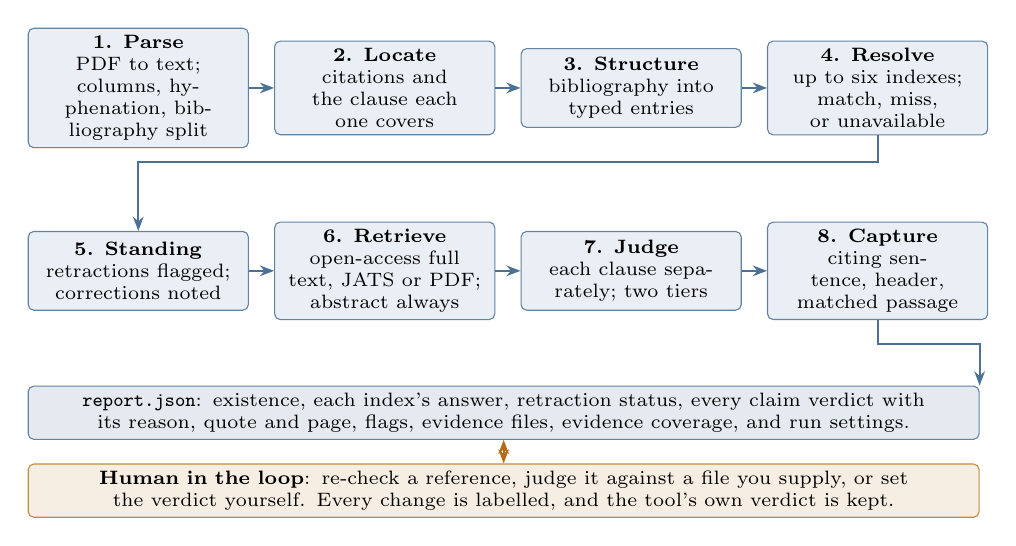
\begin{tikzpicture}[
  node distance=3.2mm,
  box/.style={
    draw=cablue!70,
    fill=calight,
    rounded corners=2pt,
    text width=2.62cm,
    minimum height=1.0cm,
    align=center,
    font=\scriptsize,
    inner sep=2.5pt
  },
  wide/.style={
    draw=cablue!70,
    fill=cablue!12,
    rounded corners=2pt,
    text width=11.9cm,
    minimum height=0.6cm,
    align=center,
    font=\scriptsize,
    inner sep=2.5pt
  },
  arr/.style={
    -{Stealth[length=1.8mm]},
    cablue!80,
    thick
  }
]

\node[box] (s1) {\textbf{1. Parse}\\ PDF to text; columns, hyphenation, bibliography split};

\node[box, right=of s1] (s2) {\textbf{2. Locate}\\ citations and the clause each one covers};

\node[box, right=of s2] (s3) {\textbf{3. Structure}\\ bibliography into typed entries};

\node[box, right=of s3] (s4) {\textbf{4. Resolve}\\ up to six indexes; match, miss, or unavailable};

\node[box, below=1.05cm of s1] (s5) {\textbf{5. Standing}\\ retractions flagged; corrections noted};

\node[box, right=of s5] (s6) {\textbf{6. Retrieve}\\ open-access full text, JATS or PDF; abstract always};

\node[box, right=of s6] (s7) {\textbf{7. Judge}\\ each clause separately; two tiers};

\node[box, right=of s7] (s8) {\textbf{8. Capture}\\ citing sentence, header, matched passage};

\node[wide, below=0.95cm of s5.south west, anchor=north west] (json)
{
\textbf{\vd{report.json}}: existence, each index's answer, retraction status, every claim verdict with its reason, quote and page, flags, evidence files, evidence coverage, and run settings.
};

\node[
  wide,
  below=3mm of json.south west,
  anchor=north west,
  draw=caamber!80,
  fill=caamber!12
] (human)
{
\textbf{Human in the loop}: re-check a reference, judge it against a file you supply, or set the verdict yourself. Every change is labelled, and the tool's own verdict is kept.
};

\draw[arr] (s1) -- (s2);
\draw[arr] (s2) -- (s3);
\draw[arr] (s3) -- (s4);

\draw[arr] (s5) -- (s6);
\draw[arr] (s6) -- (s7);
\draw[arr] (s7) -- (s8);

\draw[arr] (s4.south) -- ++(0,-0.34) -| (s5.north);
\draw[arr] (s8.south) -- ++(0,-0.3) -| (json.north east);

\draw[
  arr,
  {Stealth[length=1.8mm]}-{Stealth[length=1.8mm]},
  caamber
] (json.south) -- (human.north);

\end{tikzpicture}

\caption{
The CiteAudit pipeline. Stages 1 to 3 run once per manuscript. Stages 4 to 8 run once per reference in a small thread pool, because references can be checked independently. The checking phase has a time limit, so a publisher that stops responding delays one reference rather than the whole report.
}

\label{fig:pipeline}
\end{figure}

\subsection{Logical Architecture}

Figure~\ref{fig:logical-architecture} shows the main parts of the application and what it depends on. The browser sends the manuscript to a Flask server. The server runs the pipeline, which calls external scholarly services for metadata and source text, and writes the report and evidence to local disk. The prototype runs as one process, with no database and no external task queue.

\begin{figure}[htbp]
\centering
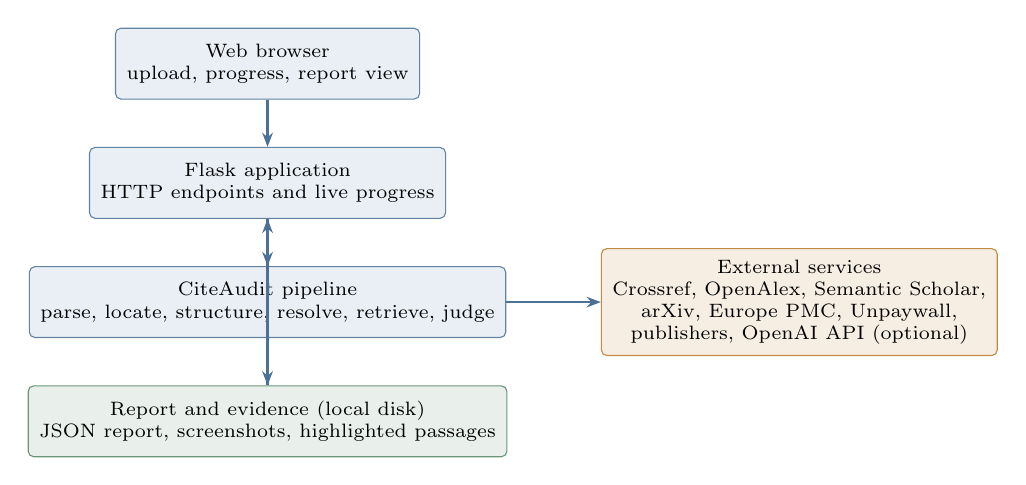
\begin{tikzpicture}[
  node distance=6mm and 8mm,
  layer/.style={draw=cablue!70, fill=calight, rounded corners=2pt, minimum width=3.1cm, minimum height=0.9cm, align=center, font=\scriptsize, inner sep=4pt},
  ext/.style={draw=caamber!80, fill=caamber!12, rounded corners=2pt, minimum width=3.1cm, minimum height=0.9cm, align=center, font=\scriptsize, inner sep=4pt},
  outputbox/.style={draw=cagreen!70, fill=cagreen!10, rounded corners=2pt, minimum width=3.1cm, minimum height=0.9cm, align=center, font=\scriptsize, inner sep=4pt},
  arr/.style={-{Stealth[length=1.8mm]}, thick, cablue!80}
]
\node[layer] (browser) {Web browser\\upload, progress, report view};
\node[layer, below=of browser] (server) {Flask application\\HTTP endpoints and live progress};
\node[layer, below=of server] (pipeline) {CiteAudit pipeline\\parse, locate, structure, resolve, retrieve, judge};
\node[ext, right=1.2cm of pipeline] (services) {External services\\Crossref, OpenAlex, Semantic Scholar,\\arXiv, Europe PMC, Unpaywall,\\publishers, OpenAI API (optional)};
\node[outputbox, below=of pipeline] (evidence) {Report and evidence (local disk)\\JSON report, screenshots, highlighted passages};
\draw[arr] (browser) -- (server);
\draw[arr] (server) -- (pipeline);
\draw[arr] (pipeline) -- (services);
\draw[arr] (pipeline) -- (evidence);
\draw[arr] (evidence.north) -| (server.south);
\end{tikzpicture}
\caption{Logical architecture of the CiteAudit prototype. The pipeline runs inside the Flask application. The scholarly indexes, publishers, and the language model are external services that the pipeline calls.}
\label{fig:logical-architecture}
\end{figure}

\subsection{Main Features}

\begin{itemize}

\item \textbf{Citation extraction with clause scoping.} Reads numeric citations such as \vd{[1]}, \vd{[1,2]}, and \vd{[1-4]}, author--year citations such as \vd{(Smith & Jones, 2019)}, and narrative citations such as \vd{Kim et al. (2021)}. It expands ranges, records the page, and assigns each citation the clause it supports. Bracketed numbers that are not citations, such as table row labels beyond the last reference, are reported separately from genuine unmatched citations.

\item \textbf{Existence checks across several indexes}: Crossref \cite{hendricks2020}, OpenAlex \cite{priem2022}, Semantic Scholar \cite{kinney2023}, arXiv, Europe PMC \cite{europepmc2015}, and Unpaywall \cite{piwowar2018}. Each index's answer is stored separately. Not every index is asked about every reference; Section~\ref{sec:sigma} gives the conditions.

\item \textbf{Retraction screening} using open retraction data \cite{crossref2023,cope2019}. Retractions, withdrawals, and removals get a high-severity flag. Corrections are shown as notes.

\item \textbf{Structural checks} for author mismatches, for example text that says ``Pinto et al.\ [29]'' when reference 29 is by Kim et al., and for the same work listed twice under different numbers.

\item \textbf{Three pieces of evidence per reference}, an abstract card when a publisher blocks automated access, and a coverage line that counts what the verdicts were based on.

\item \textbf{Re-checking and a screening result}. Any reference can be re-checked, and the report opens with one of four levels (\vd{critical}, \vd{concern}, \vd{review}, \vd{clear}) that lists the findings behind it instead of giving an opaque score \cite{hicks2015}.

\end{itemize}

\subsection{Implementation Environment}

CiteAudit is written in Python. The Docker image uses Python 3.12; the tests reported in Section~\ref{sec:results} were run on Python 3.14.6. A Flask server handles uploads and streams progress to the browser with server-sent events. References are checked in parallel with a \vd{ThreadPoolExecutor}. Most of the work is waiting for network replies, which threads handle well, so a task queue would add infrastructure without a clear benefit.

PyMuPDF reads, renders, and annotates PDFs. Using one library for both text and images keeps the extracted text and its position on the page consistent. Bibliographies are parsed with Unicode-aware regular expressions rather than GROBID \cite{lopez2009} or CERMINE \cite{tkaczyk2015}, which are more robust but would require a second runtime.

Source pages are downloaded with \texttt{requests} and parsed with BeautifulSoup and lxml. Europe PMC full text arrives as JATS XML, which is parsed directly. The word-overlap judge uses inverse document frequency (IDF) weighting and rapidfuzz; the model judge uses the OpenAI Chat Completions API (Section~\ref{sec:model}). Evidence is captured with Chromium, driven by Playwright, for web pages, and with PyMuPDF for PDFs. The front end is plain JavaScript with no build step and loads no external scripts or fonts. The tests use Python's \vd{unittest} and run offline. In Docker, the app runs under gunicorn with one worker process and 16 threads, with optional password protection. It must use a single process because the state of running jobs is kept in memory.


\section{Methodology}
\label{sec:method}

\subsection{Development Process}

We built the tool in the same order as the pipeline and tested each stage on real manuscripts before adding the next one. Development was driven by failures: every paper that broke the parser was added to a test collection, so each parsing rule exists because of a real document. Examples include non-English characters in surnames, four different author-name orders, two-column layouts, identifiers split across lines, and invisible zero-width characters that some publishers insert into DOIs.

Later we added a second rule for testing. Whenever a number or verdict changed between two runs of the same manuscript, we wrote a test for that case before fixing it. Such changes do not crash the tool, but they make it give different answers for no visible reason.

\subsection{System Workflow}

The uploaded PDF is converted to text. The tool restores the reading order of columns, rejoins hyphenated words, removes zero-width characters and running headers, and finds where the bibliography starts by searching backwards from the end of the document. It then extracts the citations and links them to bibliography entries. If a paper contains both numeric and author--year patterns, and either style has at least five citations, only the more common style is kept.

Each reference is then checked on its own in a small thread pool: the tool finds the work, checks whether it was retracted, downloads what it can, judges each claim, and takes three screenshots. A publisher can accept a connection and then never reply, so the checking phase has a time limit of $\max\{180,\ 60\,n/w\}$ seconds for $n$ references and $w$ workers. A reference that is still running at the limit is reported as \vd{unverified}, together with the step it had reached, and never as \vd{not_found}.

The report opens with the screening result, followed by one card per reference, with the cards that need the most attention first. Retracted references are placed near the top whatever their claim verdicts are. Page numbers link straight to the page in the uploaded PDF.

\subsection{Main Approach}

\subsubsection{Citation extraction and clause scoping}
\label{sec:extraction}

The text is split into sentences at full stops, question marks, and exclamation marks, ignoring common abbreviations such as ``et al.'', ``e.g.'', and ``Fig.'' and single-letter initials. Each sentence is searched for three kinds of citation: numeric, parenthetical author--year, and narrative author--year. When two matches overlap, the one that starts first and is longest wins. Numeric ranges are expanded when they span between 1 and 60 numbers, and 0 is never treated as a reference number. Capitalised words that are never surnames, such as ``Table'', ``Figure'', month names, and ``Since'', are ignored, so ``Table 2 (2019)'' is not read as a citation.

When a sentence contains several citations, each citation is given the text between the previous citation and itself. The last citation also gets the rest of the sentence, which usually holds the verb that the whole list depends on. Leading punctuation and joining words such as ``and'' are removed. If the clause has fewer than four content words, the whole sentence is used instead. The tool also records how many references are cited together at that point and passes this number to the judge.

Text that looks like a table row, heading, or caption is marked as non-prose. This happens when a span has eight or more citations, fewer than six words, fewer than 40\% of words starting with a lower-case letter, or a high share of digits and symbols. If a reference is cited both in running text and in a table, only the running-text citations are judged. In a table where at least eight citations each start their own line (at least 70\% of those whose position can be checked), the citations are treated as row labels, and each row is read forwards from its citation to the next one.

Numeric citations are linked to the entry with the same number. Author--year citations are linked through an index built from each entry's first-author surname and year. If two entries share the same surname and year, the citation is reported as unmatched rather than guessed. Numbers above the last entry are reported separately from genuinely unmatched citations, but only when the parsed entries start at 1 or 2 and cover at least 80\% of the numbers up to the last one.

\subsubsection{Existence: the exact agreement score}
\label{sec:sigma}

Each bibliography entry $r$ is first split into authors, title $t_r$, year $y_r$, venue, and any printed identifier. The tool then follows one of two paths.

\textbf{Identifier path.} If a DOI is printed, the tool looks it up in Crossref (\vd{/works/{doi}}), OpenAlex, and Europe PMC. It also asks Semantic Scholar if no abstract or open-access link has been found yet, and Unpaywall if a contact e-mail is set and no open-access link has been found yet. If an arXiv identifier is printed, the arXiv API is asked first. On this path, an index that returns the registered record counts as a match, with no title comparison.

\textbf{Title path.} If no DOI or arXiv identifier is printed, the tool searches for the printed title, or for the raw entry if no title could be parsed. A printed URL alone also follows this path. Crossref returns up to five candidates (\vd{query.bibliographic}, using the first 350 characters; skipped if the query is shorter than 12 characters), OpenAlex up to three (first 250 characters), Semantic Scholar one, and Europe PMC one (title search, used only when the title is longer than 15 characters). Every candidate is scored, not only the first, because an index does not always rank the right paper first \cite{hendricks2020}.

Titles are compared as sets of words. $T(x)$ is the set of lower-case tokens in $x$ that match \vd{[a-z0-9]{3,}}, excluding \emph{the}, \emph{and}, \emph{for}, \emph{with}, \emph{from}, \emph{into}, and \emph{using}. Title similarity is the Jaccard index
\begin{equation}
J(a,b) = \frac{|T(a) \cap T(b)|}{|T(a) \cup T(b)|}, \qquad J = 0 \text{ if either set is empty.}
\label{eq:jaccard}
\end{equation}
The agreement between the printed entry $r$ and a candidate $c$ is
\begin{equation}
s(r,c) = \min\Bigl\{1,\; J(t_r,t_c) + 0.12\,\mathbf{1}[S_r \cap S_c \neq \emptyset] + 0.08\,\mathbf{1}[y_r = y_c]\Bigr\},
\label{eq:agree}
\end{equation}
where $S$ is the set of surnames in lower case with accents removed (initials and words such as ``et al.'' are dropped), and $\mathbf{1}[\cdot]$ is 1 when its condition is true and 0 otherwise. The author and year bonuses apply to Crossref and OpenAlex candidates. Semantic Scholar and Europe PMC candidates are scored on $J$ alone. The comparison always uses the title printed in the manuscript, never a title suggested by an earlier index. Within each index, the best-scoring candidate is kept; on a tie, the one the index ranked higher wins. The best agreement across all scored candidates $\mathcal{C}(r)$ from all indexes, rounded to three decimals, is
\begin{equation}
\sigma(r) = \max_{c \in \mathcal{C}(r)} s(r,c).
\label{eq:sigma}
\end{equation}

On the title path, an index counts as a \emph{match} if its best candidate scores $s \ge 0.55$, and as a \emph{miss} otherwise. For OpenAlex and Semantic Scholar, a best candidate below 0.45 is thrown away; one between 0.45 and 0.55 still counts as a miss but may provide an abstract or an open-access link. Crossref's best candidate always provides metadata, and the report shows which title it matched and how well, with a warning when the agreement is below 0.60. A DOI found by title search is used to confirm the work in later indexes only if its Crossref agreement is at least 0.55. Otherwise a weak search result could make several indexes appear to agree on a paper the author never cited.

\textbf{Existence decision.} Let $H(r)$ be the set of indexes that matched, and $M(r)$ the set that answered without a match. An index that was unavailable belongs to neither set. It counts as unavailable if the request failed (timeout or refused connection) or if it replied with a rate-limit error (HTTP 429) or a server error (5xx). Such requests are retried up to twice first, following the service's \vd{Retry-After} header. Any other reply, such as a 404 for an unregistered DOI, counts as an answer. Then
\begin{equation}
E(r) =
\begin{cases}
\vd{confirmed} & H(r) \neq \emptyset\\[2pt]
\vd{not_found} & H(r) = \emptyset,\ M(r) \neq \emptyset, \text{ and either an identifier was printed or } \sigma(r) < 0.35\\[2pt]
\vd{unconfirmed} & \text{otherwise.}
\end{cases}
\label{eq:exist}
\end{equation}
On the title path, this gives the two thresholds shown in Figure~\ref{fig:bands}. \vd{not_found} means that none of the indexes asked returned a close enough match; it does not prove the work does not exist. We chose the thresholds (0.35 and 0.55) and the bonuses (0.12 and 0.08) during development by looking at matches on our test papers. They were not fitted to labelled data, so they are provisional and still need to be validated (Section~\ref{sec:future}). Note that the two bonuses add up to 0.20, which is exactly the width of the uncertain range.

\begin{figure}[htbp]
\centering

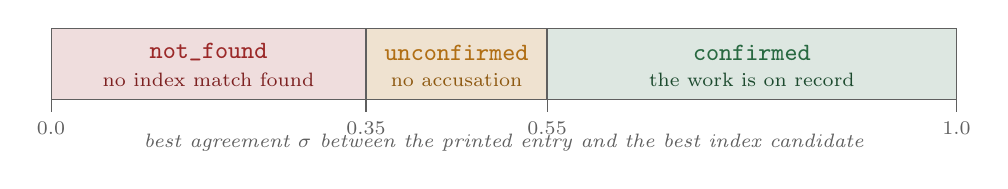
\begin{tikzpicture}[x=1cm,y=1cm]

\fill[cared!16] (0,0) rectangle (4.0,0.9);
\fill[caamber!20] (4.0,0) rectangle (6.3,0.9);
\fill[cagreen!16] (6.3,0) rectangle (11.5,0.9);

\draw[cagrey] (0,0) rectangle (11.5,0.9);

\draw[thick,cagrey] (4.0,0) -- (4.0,0.9);
\draw[thick,cagrey] (6.3,0) -- (6.3,0.9);

\foreach \x/\l in {0/0.0, 4.0/0.35, 6.3/0.55, 11.5/1.0}
    \draw[cagrey] (\x,0) -- (\x,-0.16)
    node[below,font=\scriptsize] {\l};

\node[font=\small\bfseries,cared]
at (2.0,0.60) {\vd{not_found}};

\node[font=\scriptsize,cared!80!black]
at (2.0,0.25) {no index match found};

\node[font=\small\bfseries,caamber]
at (5.15,0.60) {\vd{unconfirmed}};

\node[font=\scriptsize,caamber!80!black]
at (5.15,0.25) {no accusation};

\node[font=\small\bfseries,cagreen]
at (8.9,0.60) {\vd{confirmed}};

\node[font=\scriptsize,cagreen!70!black]
at (8.9,0.25) {the work is on record};

\node[font=\scriptsize\itshape,cagrey]
at (5.75,-0.55)
{best agreement $\sigma$ between the printed entry and the best index candidate};

\end{tikzpicture}

\caption{
The existence decision on the title path. In the middle range the tool makes no claim and asks a person to check. A real paper with an unusual title, venue, or type can land here instead of being reported as missing.
}

\label{fig:bands}

\end{figure}

Retractions are detected from three sources: Crossref update records (\vd{updated-by} entries of type retraction, withdrawal, or removal) \cite{crossref2023}, the OpenAlex \vd{is_retracted} flag \cite{priem2022}, and Europe PMC correction entries of a retraction type. Retracted papers are shown near the top of the report, because a retracted source cannot reliably support a claim \cite{hsiao2021,schneider2020}. Corrections are only noted: a corrected paper is still the cited work, and a correction does not mean the citation is wrong \cite{cope2019}.

\subsubsection{Retrieval and coverage recording}

For each reference, the tool tries three addresses in order: the open-access link (from arXiv, OpenAlex, Semantic Scholar, Unpaywall, or Europe PMC), then the resolved URL, then the landing page. It keeps the first reply that has more than 600 characters of text and does not look like a paywall. Downloads are capped at 12\,MB, and at most 40 PDF pages are read. The abstract from the index is always part of the text that is judged. If less than 400 characters were retrieved, the abstract is used instead; otherwise it is added at the start if it is not already there.

The report records what kind of content was retrieved for each reference, in five categories: \emph{full text} (PDF or Europe PMC XML), \emph{publisher or landing page} (an HTML page, which may or may not contain the full article), \emph{abstract only}, \emph{document supplied by the user}, and \emph{nothing retrieved}. The counts appear under the screening result, so a reader can tell ``nothing wrong was found'' apart from ``little could be checked''.

\subsubsection{Claim scoping and two-tier judging}

One sentence can make several claims, each backed by a different source. For example:

\emph{
``parameters such as soil moisture [37], field temperature [38] and crop yield [39] can all be predicted.''
}

If the whole sentence were sent to all three sources, each source would be asked to support all three claims, and one correct sentence could produce three false negative findings. Each citation is therefore judged on its own clause, with the full sentence kept as context. If the clause is too short to stand alone (fewer than four content words), the whole sentence is used. In this example, [37] and [38] fall back to the whole sentence, while [39] is judged on ``crop yield can all be predicted''.

When a reference is cited both in a table and in the running text, the running text is judged, because a table row such as ``Ref.\ Method Year Dataset'' gives the judge too little to work with. Judging each claim separately is what separates claim-level auditing from simple reference checking \cite{ref2,ref8}, and it follows the setup used in claim-verification research \cite{wadden2020,thorne2018}.

Judging has two tiers (Table~\ref{tab:verdicts}). The word-overlap (lexical) tier always runs. The claim and the source are split into lower-case words, with stop words removed and common endings stripped. The source is split into passages of about 320 characters, and the title and abstract form one extra passage. With $N$ passages and $\mathrm{df}(t)$ the number of passages that contain word $t$,
\begin{equation}
\mathrm{idf}(t) = \ln\!\Bigl(1 + \frac{N}{1 + \mathrm{df}(t)}\Bigr),\qquad
g(C,P) = 0.68\,\frac{\sum_{t \in C \cap P} \mathrm{idf}(t)}{\sum_{t \in C} \mathrm{idf}(t)} + 0.32\,f(C,P),
\label{eq:lexical}
\end{equation}
where $f$ is the rapidfuzz token-set similarity, scaled to $[0,1]$. A claim's score mixes its best passage with the average of its best three: $\ell = 0.72\,g_{(1)} + 0.28\,\bar g_{(1:3)}$. Scores of at least 0.52, 0.34, and 0.18 give \vd{supported}, \vd{related}, and \vd{weak}; lower scores give \vd{unverified}. These weights and cut-offs were set by hand during development. The optional model tier is described in Section~\ref{sec:model}.

We keep both tiers because the model is not always available: the API key may be missing, a request may be rejected, or the account may hit a rate limit, and the tool should still give a basic result. The lexical tier also finds the matching passage in the source, which the screenshot step needs for highlighting.

\begin{table}[htbp]
\centering

\caption{
The verdicts. Low word overlap does not always mean a claim is unsupported: ``in the early stages they had military purposes [1]'' may share few words with an abstract that fully supports it. For this reason, the lexical tier never returns \vd{unrelated}, and without a model the lowest verdict is \vd{unverified}.
}

\label{tab:verdicts}

\small

\begin{tabularx}{\textwidth}{@{}l X l@{}}

\toprule

\textbf{Verdict}
&
\textbf{Meaning}
&
\textbf{Given by}
\\

\midrule

\vd{supported}
&
The source directly supports the claim.
&
both tiers
\\

\vd{related}
&
The source is on the same topic and consistent with the claim, but does not state it.
&
both tiers
\\

\vd{weak}
&
The source is only loosely connected to the claim.
&
both tiers
\\

\vd{unrelated}
&
The source is about something else.
&
\textbf{model tier only}
\\

\vd{unverified}
&
Not enough text was retrieved to decide.
&
both tiers
\\

\vd{not_found}
&
None of the indexes asked returned a close enough match for the reference.
&
existence check
\\

\bottomrule

\end{tabularx}

\end{table}

\subsubsection{Model tier configuration}
\label{sec:model}

Table~\ref{tab:model} gives the full configuration of the model tier as it is implemented. The system instruction, the prompt template, and the output schema are part of the released source code (Section~\ref{sec:privacy}).

\begin{table}[htbp]
\centering
\caption{Model tier configuration, as implemented in \vd{citecheck/match.py}.}
\label{tab:model}
\small
\begin{tabularx}{\textwidth}{@{}>{\raggedright\arraybackslash}p{3.3cm} X@{}}
\toprule
\textbf{Item} & \textbf{Setting}\\
\midrule
Provider and API & OpenAI Chat Completions with structured outputs, through the OpenAI Python SDK. Any OpenAI-compatible endpoint can be used by setting \vd{OPENAI_BASE_URL}.\\
\addlinespace
Model & Set with \vd{CITECHECK_OPENAI_MODEL}; the code default is \vd{gpt-4o}. The installation used for all runs in this paper is set to \vd{gpt-4.1}; its configuration file was last changed on 31 July 2026, before any of the runs. The model is called by name, not by a dated snapshot. The four operating runs date from 6 August to 1 September 2026, and the benchmark from 21 September 2026. Every report now records the model name and the start time (\vd{stats.run_config}).\\
\addlinespace
When it runs & When an API key is set, the SDK is installed, \vd{CITECHECK_LLM} is not \vd{off}, and the user has not turned model judging off for the run.\\
\addlinespace
Prompt & System instruction: judge only from the text supplied, read the abstract first, use \vd{unrelated} only for a different subject, prefer \vd{unverified} when the text is too thin, and quote word for word. User message, in this order: the claim clause; the full sentence if it differs, with a note that the rest belongs to the other cited sources; a note when several sources are cited together; the reference as printed; the retrieved title; the abstract under its own heading; and the first 24{,}000 characters of retrieved text.\\
\addlinespace
Output & A strict JSON schema with four required fields: \vd{verdict} (\vd{supported}, \vd{related}, \vd{weak}, \vd{unrelated}, or \vd{unverified}), \vd{confidence} (0--1), \vd{reason} (one or two sentences), and \vd{evidence_quote} (a word-for-word quote, or empty).\\
\addlinespace
Sampling & Temperature 0, top-$p$ 1, seed 20240516. If a model rejects these settings, the call is repeated once without them.\\
\addlinespace
Limits & At most six claims per reference are sent (1--20 for re-checks). No call is made if both the retrieved text and the abstract are shorter than 120 characters.\\
\addlinespace
Negative verdicts & A \vd{weak} or \vd{unrelated} verdict is judged again against the abstract alone. If the second verdict is milder, it replaces the first, and the claim is marked as reconsidered.\\
\addlinespace
Failures & If a request fails, is refused by the content filter, or returns output that cannot be read, that claim gets no model verdict and is kept as \vd{unverified} rather than dropped. If no call for a reference succeeds, the lexical result is used and its reason says why. The report header names the tier that actually produced the verdicts and how many references it judged.\\
\addlinespace
Combining claims & Model tier: the most serious claim verdict. Lexical tier: the best one, because low overlap is not evidence against a source.\\
\bottomrule
\end{tabularx}
\end{table}

Temperature 0 and a fixed seed make repeated calls give the same answer for the same model version. At default settings, the same claim and text could come back \vd{related} on one call and \vd{weak} on the next. However, a hosted model behind the same name can be updated, so results may still change over time.

\vd{unrelated} and \vd{weak} are negative findings, so the tool is careful before reporting them. A common cause of a wrong negative verdict is judging text in which the abstract is buried or missing. The abstract is therefore always sent separately, and every negative verdict is checked again against the abstract alone before it is reported \cite{ji2023}.

When a reference has several claim verdicts, the model tier reports the most serious one, because one unsupported claim still matters. The lexical tier reports the best one, because low word overlap alone does not show that a claim is unsupported.

\subsection{Implementation}

The code has 6{,}801 lines of Python: the Flask server (575 lines) and nine pipeline modules with a package file (6{,}226 lines). There are also 2{,}360 lines of tests and 410 lines of benchmark and evaluation tools. Uploads are limited to 60\,MB. By default, a run checks up to 250 references (configurable from 1 to 500), four at a time (configurable from 1 to 8), and sends at most six claims per reference to the model, which keeps the cost of heavily cited references under control.

The tool does not bypass CAPTCHAs or consent pages. When a publisher shows one, the report says so and shows a labelled abstract card instead. Each worker thread keeps one browser open and uses a fresh browser context for each reference. PDF highlighting works on normalised word positions, so matches still work across line breaks, columns, and hyphenated words.

The two actions that change a saved report, re-check and manual verdict, cannot run at the same time. Each one updates a single entry and sends back only that entry and the recomputed summary. If a re-check retrieves nothing, the earlier result is kept. If it does retrieve text, any verdict set by hand on that reference is cleared, and the report says so.

\subsection{Checking the Paper Against the Code}
\label{sec:trace}

We checked every mechanism described in this paper against the source code of the version described here. Table~\ref{tab:trace} shows where each one is implemented and which offline tests cover it. The concurrency benchmark (Section~\ref{sec:concurrency}) also exposed one bug in the code, which we fixed before producing the results reported there.

\begin{table}[htbp]
\centering
\caption{Where each mechanism is implemented. Every entry was confirmed by reading the code. ``Tests'' names the offline test module that covers the behaviour.}
\label{tab:trace}
\small
\begin{tabularx}{\textwidth}{@{}>{\raggedright\arraybackslash}p{3.4cm} >{\raggedright\arraybackslash}X >{\raggedright\arraybackslash}p{3.0cm}@{}}
\toprule
\textbf{Mechanism} & \textbf{Where implemented} & \textbf{Tests}\\
\midrule
Citation extraction & \vd{intext.extract_citations}, \vd{_markers_in}, \vd{_expand_numeric}; majority-style rule & \vd{test_styles}, \vd{test_claims}\\
Clause scoping & \vd{intext._clause_for} (four-content-word fallback; row labels read forwards) & \vd{test_claims}\\
Linking citations to entries & \vd{refs.index_references}, \vd{refs.link_citations}; \vd{pipeline._split_out_of_range} & \vd{test_styles}, \vd{test_corpus}\\
Six-index lookup & \vd{resolve.resolve}: Crossref, OpenAlex, Semantic Scholar, arXiv, Unpaywall, Europe PMC (conditional) & needs live services; not covered offline\\
Existence score & \vd{resolve._agreement}, \vd{_title_agreement}, \vd{_settle_existence}; thresholds 0.55 and 0.35 & no unit test; checked against stored reports (Section~\ref{sec:operating})\\
Unavailable-index rule & \vd{resolve._get} (retry on 429, 502, 503, 504), \vd{resolve._record} (429 and 5xx counted as unavailable) & \vd{test_reporting_additions}\\
Retraction checking & \vd{resolve._apply_crossref_integrity}, OpenAlex \vd{is_retracted}, Europe PMC corrections & \vd{test_report}, \vd{test_stability} (reporting only)\\
Two-tier judging & \vd{match.lexical_match}, \vd{match.judge}, \vd{openai_match}, \vd{_second_look}, \vd{roll_up} & \vd{test_claims}, \vd{test_stability}\\
Evidence capture & \vd{shots.capture_citing}, \vd{shots.capture}, \vd{render_abstract_card} & not covered offline\\
Coverage recording & \vd{pipeline.coverage}, \vd{coverage_of} & \vd{test_reporting_additions}\\
Human override & \vd{pipeline.set_verdict}, \vd{_settle_headline}, \vd{recheck_one} & \vd{test_claim_recheck}, \vd{test_stability}\\
Threads and time limit & \vd{pipeline.run} (\vd{ThreadPoolExecutor}, \vd{as_completed} with a time limit); \vd{app._RECHECK_LOCK} & \vd{test_stability}\\
Retention and deletion & \vd{app.purge_expired}, \vd{DELETE /api/run/<id>} & \vd{test_reporting_additions}\\
\bottomrule
\end{tabularx}
\end{table}


\section{Evaluation}
\label{sec:eval}

\subsection{Evaluation Setup}

We evaluated CiteAudit in three ways. First, an automated test suite that runs offline: every document, index reply, report, and bibliography the tests need is stored with the tests, so the results do not depend on live services or an API key. Second, measurements from the reports of four published manuscripts processed end to end with live services (Section~\ref{sec:operating}). Third, a benchmark with several manuscripts running at the same time (Section~\ref{sec:concurrency}).

The tests use two kinds of input: synthetic bibliographies that cover the supported styles, and real published articles that once broke the parser. The real articles are copyrighted and are not shared; their tests are skipped when the files are missing.

\subsection{Evaluation Criteria}

\begin{itemize}

\item \textbf{Format coverage}: are bibliographies and citations parsed correctly across the main citation styles and author-name orders \cite{lopez2009,tkaczyk2015}?

\item \textbf{Clause scoping}: does each citation get the right clause, and does re-checking one citation leave the others unchanged?

\item \textbf{Reporting correctness}: does the screening result follow from the findings, and is a run that checked nothing never reported as clean?

\item \textbf{Stability}: does the same manuscript give the same numbers and verdicts when checked twice?

\item \textbf{Runtime}: how long does a manuscript take, per manuscript and per reference, and with or without the model?

\item \textbf{Existence outcomes and coverage}: what share of references falls in each existence outcome, and what kind of content was each verdict based on?

\item \textbf{Behaviour under load}: what happens to speed, failures, and result quality when several manuscripts run at once?

\end{itemize}

We treat stability as a main criterion. An inconsistent result does not crash anything, but a reader notices it at once, and it quickly erodes trust in the tool.

\subsection{Results}
\label{sec:results}

\textbf{Test suite.} The suite has 192 tests, all passing, in 6.5 seconds on Python 3.14.6 under Windows~11, with no network access. It contains 65 stability tests, 50 tests of clause scoping and citation precision, 26 tests checking that re-checking one citation leaves the others unchanged, 22 tests of bibliography and citation styles, 8 tests on real papers that once broke the parser, 5 tests of the screening result (including the empty-run case), and 16 tests of evidence coverage, run settings, retention and deletion, the evaluation metrics, and the handling of throttled index replies.

The style tests cover APA, Harvard, Vancouver, IEEE, ACM, Nature, Chicago, MLA, and Elsevier/Springer numbered styles, four author-name orders, accented and double-barrelled surnames, two-column layouts, and identifiers split across lines.

Stability tests are the largest group, which shows where much of the engineering work went. Each one records a case where a number or verdict changed even though the citation had not. Examples include a summary that counted references while the cards counted citations, a claim that disappeared from the result when its model call failed, and a re-check that found no text but still replaced a verdict based on real text.

\subsection{Operating Measurements on Four Manuscripts}
\label{sec:operating}

We processed four published manuscripts end to end through the web interface between 6~August and 1~September 2026, with model judging and evidence capture turned on. All numbers below were recomputed from the saved \vd{report.json} files of those runs. M1 is a 17-page wireless networking article, M2 a 20-page security games article, M3 a 25-page networking review, and M4 a 55-page transport safety review. M1 to M3 are also in our test collection, so they are development documents, not an independent sample. We identify them only by type, because the outcomes are unverified tool outputs, not findings about their authors.

Three points should be kept in mind. First, the runs used versions of the code from 6~August to 1~September. The existence-scoring code has not changed since 6~August, but M1 to M3 were judged before clause scoping was added on 20~August, so their claim counts come from sentence-level judging. Second, those reports did not record the number of workers; the default is four. Third, 40 references of M4 were later re-checked against documents supplied by a person, so M4 is left out of the coverage figures.

\begin{table}[htbp]
\centering
\caption{Measurements on four manuscripts, recomputed from the saved reports. The existence outcomes are tool outputs and were not checked against independent labels.}
\label{tab:operating}
\small
\begin{tabular}{@{}l r r r r r@{}}
\toprule
& \textbf{M1} & \textbf{M2} & \textbf{M3} & \textbf{M4} & \textbf{Total}\\
\midrule
Pages & 17 & 20 & 25 & 55 & 117\\
Citations found & 38 & 25 & 204 & 413 & 680\\
References checked & 36 & 24 & 149 & 155 & 364\\
Claims judged & 34 & 16 & 175 & 219 & 444\\
Model tier on & yes & yes & yes & yes & \\
Processing time (s) & 156.6 & 83.7 & 783.3 & 751.8 & 1{,}775.4\\
Seconds per reference & 4.4 & 3.5 & 5.3 & 4.9 & 4.9\\
\midrule
Existence: confirmed & 34 & 16 & 137 & 142 & 329\\
Existence: unconfirmed & 0 & 0 & 8 & 7 & 15\\
Existence: no index match & 2 & 8 & 4 & 6 & 20\\
Author-mismatch / duplicate flags & 1 / 1 & 0 / 0 & 0 / 0 & 4 / 1 & 5 / 2\\
\midrule
Evidence: page capture & 20 & 10 & 69 & 68 & 167\\
Evidence: abstract card & 13 & 8 & 67 & 87 & 175\\
Evidence: no passage capture & 3 & 6 & 13 & 0 & 22\\
\bottomrule
\end{tabular}
\end{table}

\textbf{Runtime.} Each manuscript took between 1.4 and 13.1 minutes, or 3.5 to 5.3 seconds per reference, and the time grew roughly in line with the number of references. No reference hit the time limit. In M3 and M4, the model judged 279 of the 289 references that had retrievable text (96.5\%); the rest fell back to the lexical tier. The M1 and M2 reports were made before this figure was recorded.

\textbf{Existence.} Of the 364 references, 329 (90.4\%) were confirmed in at least one index, 15 (4.1\%) were left unconfirmed, and 20 (5.5\%) had no index match. Fifteen references printed an identifier (12 DOIs, 2 URLs, and 1 arXiv identifier); the rest were found by title search. The saved scores agree with Equation~\eqref{eq:exist}: every reference without a match had $\sigma \le 0.333$, and 14 of the 15 unconfirmed references fell inside the uncertain range ($0.375 \le \sigma \le 0.538$). The fifteenth was a book chapter whose parsed title was too short to search, so no index was asked about it. It stayed unconfirmed with $\sigma = 0$, as the rule requires. None of these references was checked by hand, so the 20 references without a match are candidates for checking, not proven fabrications.

\textbf{Evidence coverage.} Table~\ref{tab:coverage} shows what was retrieved for the 209 references of M1 to M3. Full text (JATS XML or PDF) was found for 28 references (13.4\%). Another 32 (15.3\%) gave an HTML page with readable text. The median length of these pages was 2{,}299 to 9{,}419 characters per manuscript, against 32{,}735 and 59{,}004 characters for the PDFs of M1 and M3, so most were landing pages or partial pages. The largest group, 123 references (58.9\%), was judged on the abstract alone, and nothing usable was found for 26 (12.4\%), including 11 publisher pages that returned no readable text. Most claims were therefore judged on abstracts. A matched-passage screenshot or an abstract card was produced for 342 of the 364 references (94.0\%), the citing sentence was captured for 360 (98.9\%), and the source header for 314 (86.3\%).

\begin{table}[htbp]
\centering
\caption{Content retrieved per reference for M1 to M3, using the same categories the reports now use (\vd{pipeline.coverage_of}). A page with no readable text counts as no usable content. Shares are rounded.}
\label{tab:coverage}
\small
\begin{tabular}{@{}l r r r r r@{}}
\toprule
\textbf{Content retrieved} & \textbf{M1} & \textbf{M2} & \textbf{M3} & \textbf{Total} & \textbf{Share}\\
\midrule
Full text: JATS XML & 2 & 0 & 13 & 15 & 7.2\%\\
Full text: PDF & 1 & 0 & 12 & 13 & 6.2\%\\
Publisher or landing page (HTML) & 5 & 10 & 17 & 32 & 15.3\%\\
Abstract only & 24 & 6 & 93 & 123 & 58.9\%\\
No usable content & 4 & 8 & 14 & 26 & 12.4\%\\
\midrule
Total & 36 & 24 & 149 & 209 & 100\%\\
\bottomrule
\end{tabular}
\end{table}

\textbf{Structural checks.} The runs raised five author-mismatch flags and two duplicate-entry flags. None of the cited works had a retraction notice.

\subsection{Concurrent Use and Scalability}
\label{sec:concurrency}

\textbf{Setup.} We measured concurrent use with the benchmark included in the release (\vd{tools/benchmark.py}) on 21~September 2026. At each level $k \in \{1, 2, 5, 10\}$, $k$ runs started at the same moment on separate threads of one process, which is how the server handles $k$ uploads at once. The runs alternated between M1 (36 references) and M2 (24 references). Every run used the default settings: four workers, model judging with \vd{gpt-4.1}, and evidence capture. No contact e-mail was set, so Unpaywall was not used and the scholarly indexes were queried anonymously. The machine was a laptop with an AMD Ryzen~7 5825U processor (8 cores, 16 threads) and 15.3\,GB of memory, running Windows~11 and Python 3.14.6 on a home internet connection. Each level was run once, so the results show the trend, not the variation between runs.

\begin{table}[htbp]
\centering
\caption{Concurrency benchmark on the fixed code. Latency is the time one run takes from start to finished report. ``Judged by model'' counts references with retrievable text that received a model verdict.}
\label{tab:concurrency}
\small
\begin{tabular}{@{}l r r r r@{}}
\toprule
\textbf{Runs at the same time} & \textbf{1} & \textbf{2} & \textbf{5} & \textbf{10}\\
\midrule
References checked (all runs) & 36 & 60 & 156 & 300\\
Total time for the level (s) & 195.4 & 223.1 & 361.6 & 511.8\\
Median run latency (s) & 195.4 & 186.3 & 359.4 & 438.0\\
Median latency, M1 / M2 (s) & 195.4 / -- & 223.1 / 149.6 & 361.0 / 254.8 & 511.3 / 357.7\\
Throughput (references per minute) & 11.1 & 16.1 & 25.9 & 35.2\\
Failed runs & 0 & 0 & 0 & 0\\
References that hit the time limit & 0 & 0 & 0 & 1\\
\midrule
Judged by model & 33/33 & 48/49 & 99/101 & 180/227\\
\quad share & 100\% & 98.0\% & 98.0\% & 79.3\%\\
References with a rate-limited model call & 0 & 0 & 0 & 44\\
\midrule
Existence: confirmed & 35 & 51 & 110 & 237\\
Existence: unconfirmed & 0 & 1 & 34 & 26\\
Existence: no index match & 1 & 8 & 12 & 36\\
No usable content & 3 (8.3\%) & 11 (18.3\%) & 55 (35.3\%) & 73 (24.3\%)\\
\bottomrule
\end{tabular}
\end{table}

\textbf{Results.} Table~\ref{tab:concurrency} shows the results. No run failed at any level, and only one reference out of 300 hit the time limit, at ten runs. Throughput rose from 11.1 to 35.2 references per minute, but more slowly than the load: ten runs at once took 2.6 times as long as one, and the slowest M1 run took 511.8 seconds, against 195.4 seconds alone.

The quality of the results dropped before anything failed. At ten runs, the model provider rejected calls for 44 references because of its rate limit. Those references fell back to the lexical tier, as designed, and the share judged by the model fell to 79.3\%. The scholarly indexes and publishers also slowed down or refused requests, so the share of references with no usable content rose from 8.3\% for one run to between 18.3\% and 35.3\% under load. References whose indexes were unavailable were reported as \vd{unconfirmed} (up to 34 at five runs, against none for a single run). Importantly, neither manuscript ever received more \vd{not_found} results under load than when it ran alone (at most one per M1 run and seven per M2 run). This is what the existence rule is meant to guarantee.

\textbf{A bug found by the benchmark.} Our first pass of the benchmark showed that the rule in Section~\ref{sec:sigma} was not fully implemented. When an index replied with a rate-limit error (HTTP 429) or a server error (5xx), the code treated the reply as ``no match'' instead of ``unavailable''. Under load, this turned real references into \vd{not_found}. At ten runs, 69 of 300 references were reported as having no match, against 35 to 45 expected from the single runs. In one M1 run, six references that Crossref and OpenAlex had confirmed when the manuscript ran alone were among them. We changed the code to treat these replies as unavailable and to retry them up to twice (Section~\ref{sec:sigma}), added four offline tests, and repeated the whole benchmark. Table~\ref{tab:concurrency} shows only the repeated run.

The four manuscripts in Section~\ref{sec:operating} were each run on their own, and all their \vd{not_found} references had $\sigma \le 0.333$. However, they were run before this fix, so we cannot rule out that a throttled reply affected some of them. This is one more reason to treat those 20 references as candidates for checking, not as findings.

\textbf{What this means.} On this laptop, the prototype handles ten manuscripts at once without failing, but the results under load are not as good as when a manuscript runs alone: fewer model verdicts, less retrieved text, and more unconfirmed references. The limits come from external rate limits, not from the machine. A deployment that expects several submissions at once would need a queue that limits how many runs start together, a contact e-mail so that the scholarly indexes can identify the caller, and a model account with a rate limit that matches the load. The benchmark covers one machine, two manuscripts, and one pass per level. It does not measure a multi-user server over a network, memory use, or larger manuscripts under load.

\subsection{Accuracy: Current Status}
\label{sec:accuracy}

This paper reports no accuracy figures, because no manually labelled dataset exists yet. Without one, we cannot compute precision, recall, linking accuracy, clause-scoping accuracy, existence error rates, or agreement with human reviewers. We have not estimated any of these from the tests or the runs.

The release includes a scoring tool (\vd{tools/evaluate.py}) for the labelled study described in Table~\ref{tab:protocol}. It exports one row per citation from a run report, with the tool's answers filled in. Annotators then add their own labels: whether the row is a real citation, which reference it should point to, whether the clause is right, whether the reference exists, and whether the source supports the claim. They also add rows for citations the tool missed. The tool then computes citation precision and recall, linking accuracy, clause-scoping accuracy, an existence confusion matrix with the false no-match rate, and claim-support accuracy and Cohen's $\kappa$, both overall and by type of evidence. With a second annotator's labels, it also computes agreement between the two annotators. It reports nothing for a metric that has no labelled rows.

\subsection{Limits of the Current Evaluation}

The 192 tests check regressions and stability; they are not an accuracy benchmark. They support claims about supported formats, consistent behaviour, the rules behind the screening result, and repeatability. They do not support any claim about precision, recall, F1, false positives, or agreement with humans for citation extraction, linking, clause scoping, reference lookup, or claim judging. The measurements on four manuscripts show speed, existence outcomes, and coverage, but not whether those outcomes are correct. The concurrency benchmark covers one machine, two manuscripts, and one pass per level (Section~\ref{sec:concurrency}).

\subsection{Comparison with Existing Tools}

Table~\ref{tab:compare} compares CiteAudit with the systems in Section~\ref{sec:related} by what they can do, not by accuracy. These systems answer related but different questions, and no shared benchmark covers all of them \cite{thorne2018,wadden2020,vladika2023}.

\begin{table}[htbp]
\centering

\caption{
Capability comparison, based on each system's published description. Yes: the capability is described. No: it is only partial, outside the described scope, or not described.
}

\label{tab:compare}

\small

\setlength{\tabcolsep}{4pt}

\begin{tabular}{@{}l c c c c c@{}}

\toprule

\textbf{Capability}
&
\textbf{BibAgent}
&
\textbf{GhostCite}
&
\textbf{SemanticCite}
&
\textbf{DeepTRACE}
&
\textbf{CiteAudit}
\\

\midrule

Existence check across several indexes
&
Yes & Yes & No & No & Yes
\\

Retraction screening
&
No & No & No & No & Yes
\\

Checking whether each claim is supported
&
Yes & No & Yes & Yes & Yes
\\

Clause-level citation scoping
&
No & No & No & No & Yes
\\

Structural checks
&
No & No & No & No & Yes
\\

Strategy for paywalled sources
&
Yes & No & No & No & Yes
\\

Visual evidence capture
&
No & No & No & No & Yes
\\

Explicit uncertain outcome
&
No & No & Yes & No & Yes
\\

Labelled human override
&
No & No & No & No & Yes
\\

Works on an uploaded manuscript
&
Yes & Yes & No & No & Yes
\\

\bottomrule

\end{tabular}

\end{table}

Existence checking and claim judging already exist in other systems, but usually in separate tools. What CiteAudit adds is retraction screening, clause-level scoping, structural checks, visual evidence, and a labelled human override, all in one tool that works on a single manuscript. These are the features that make a report quick for an editor to check. Index-scale systems \cite{nicholson2021,peroni2020} and citation intent classifiers \cite{cohan2019,jurgens2018} answer different questions and complement this work.

\subsection{Worked Example}

This example follows one reference of M1 through the pipeline, as recorded in the saved report. The manuscript cites \vd{[1, 2]} on page 1, in a sentence that begins ``Although in the early stages they had military purposes''. Reference 1 is a 2005 conference paper with a printed DOI, so the identifier path was used. Crossref and OpenAlex returned the registered record, and Europe PMC answered without a match, so the reference was \vd{confirmed}. It had no retraction or correction notice. The full text could not be retrieved, so the claim was judged against the abstract (1{,}243 characters). The model returned \vd{supported} with confidence 0.90, explaining that the source traces the history of unmanned aircraft back to their military origins, and quoted a sentence from the abstract. The report stores the citing sentence highlighted on page 1, the header of the publisher's page, and the matching sentence highlighted on that page. The same manuscript also produced the structural findings used as examples in Section~\ref{sec:tool}: its text credits ``Pinto'' for reference 29, which is by Kim et al., and its reference 34 is a duplicate of reference 29. This is a recorded output, not an accuracy result.

\section{Discussion}
\label{sec:discussion}

\subsection{Main Findings}

Four findings stand out. First, what the tool can find out is limited mainly by what it can retrieve, not by how it judges. In the three manuscripts analysed for coverage, 58.9\% of references were judged on the abstract alone and only 13.4\% on full text (Table~\ref{tab:coverage}).

Second, most of the difficulty comes before the claim is judged: getting clean text out of two-column PDFs, working out which reference a citation points to, and making sure the retrieved work is really the cited one. Claim judging is only the visible end of the pipeline \cite{thorne2018,wadden2020}.

Third, clause scoping was an important design choice, because it stops one sentence with several citations from being treated as if every source had to support every claim. The tests confirm that scoping behaves as specified, but we have not yet measured how much it improves accuracy.

Fourth, keeping the output stable took a lot of work, and the uncertain range did its job in practice. Of the 192 tests, 65 (33.9\%) are stability tests, which check repeatability, not accuracy. In the four manuscripts, 15 of 364 references (4.1\%) were held back from any accusation and left for a person to check.

\subsection{Advantages}

CiteAudit brings together checks that are usually spread across several tools, and it works on a manuscript before publication rather than on published collections \cite{nicholson2021,peroni2020}. It gives verdicts per claim, which is the level at which an author would actually fix a citation \cite{ref2}: a reference that supports three of the four statements it is cited for produces one specific finding instead of a single verdict on the whole entry. Every finding comes with its evidence (the citing sentence, the source header, and the matching passage) rather than a score, so a reader can check the tool instead of simply trusting it \cite{hicks2015}.

Two more properties come from the error policy. Because a false accusation counts as worse than a missed fabrication, the tool fails quietly: a reference it cannot find is reported as unconfirmed, not fabricated. And because every result can be overridden and every override is labelled, a report that is clean because a person marked it clean cannot be confused with one that is clean on the tool's own findings.

\subsection{Limitations}

Retrieval limits everything that comes after it. For bibliographies drawn mostly from commercial publishers, many sources give only an abstract, and judging a specific claim against an abstract is much weaker than judging it against the full paper. Open access also varies a lot between fields and venues \cite{piwowar2018}. The report shows what was retrieved for each reference, so a weakly checked reference is visible as such.

Two parts of the tool have their own limits. The bibliography parser is rule-based: tests cover nine styles, but real bibliographies vary widely, and machine-learning extractors are more robust at the cost of a second runtime \cite{lopez2009,tkaczyk2015}. When parsing finds nothing, the report says so instead of showing an empty result as clean. The model tier shares the weaknesses of language models \cite{ji2023,liang2024}. Fixed sampling and the second reading of negative verdicts make it consistent and cautious, but not necessarily correct, and a hosted model can change between runs. An unconfirmed reference is still judged against the best candidate found, which may be a different paper; its card shows how well that candidate matched.

Index coverage is uneven, and that matters. Books, theses, standards, non-English work, and regional journals are found less reliably, because they are less well indexed, not because they are less real \cite{bornmann2015}. A manuscript that cites many such works will collect unconfirmed results that reflect gaps in the indexes, not poor citation practice.

The existence thresholds, the author and year bonuses, and the lexical weights were set by judgement, not fitted to data, and accuracy has not yet been measured against labelled data (Section~\ref{sec:accuracy}). Under heavy load, rate limits at the model provider and at the indexes reduce model coverage and retrieved text, although no run failed at ten simultaneous runs (Section~\ref{sec:concurrency}).

Finally, the tool checks whether citations are \emph{accurate}, not whether they are \emph{appropriate}. Whether a citation is the right one to use, whether better support exists, or whether important opposing work was left out are questions it cannot answer \cite{hicks2015,jurgens2018}.

\subsection{Privacy, Security, and Reproducibility}
\label{sec:privacy}

Uploaded manuscripts may be unpublished or confidential. This is how the prototype handles them.

\begin{itemize}
\item \textbf{What happens to an upload.} The PDF is saved on the server in an \vd{uploads} folder under a run identifier generated by the server. The pipeline reads it locally, and the report (\vd{report.json}) and evidence images, which include screenshots of the manuscript's own pages, are saved in a folder for that run.

\item \textbf{How long it is kept.} By default, uploads and run folders are kept until someone deletes them. If \vd{CITECHECK_RETENTION_HOURS} is set, every finished run, with its manuscript, report, and images, is deleted that many hours after it was last used. The clean-up runs when the server starts and on every upload, and it never touches a run in progress. A single run can be deleted at once with \vd{DELETE /api/run/<run_id>}. Progress data held in memory is lost when the server stops.

\item \textbf{What is sent to scholarly services.} Search queries built from the reference list (titles, authors, DOIs, and arXiv identifiers of the cited works) are sent to Crossref, OpenAlex, Semantic Scholar, arXiv, and Europe PMC, and to Unpaywall when a contact e-mail is set, together with that e-mail. Download requests go to publishers and open-access sites, and the screenshot browser loads their pages. The manuscript file itself is never sent to these services.

\item \textbf{What is sent to the language model.} Only when model judging is on: for each judged claim, the claim, its citing sentence, the printed reference, the retrieved title and abstract, and up to 24{,}000 characters of retrieved source text are sent to the configured OpenAI-compatible endpoint. The full manuscript is not sent, but its citing sentences are. How long the provider keeps this data depends on the provider's policy, which this paper does not cover. With model judging off, nothing is sent to a model.

\item \textbf{Access and security.} Setting \vd{CITECHECK_PASSWORD} puts one shared password in front of every page, using HTTP basic authentication with a constant-time comparison. Without it, the app is open and should only run on \vd{127.0.0.1}. There are no user accounts, so anyone with the password who knows a run identifier can open that run. Run identifiers are generated by the server and checked against a fixed pattern, uploaded file names are cleaned, and uploads are limited to 60\,MB. The prototype has no HTTPS of its own (it must sit behind HTTPS when reachable over a network), no encryption of stored files, and no audit log, and it has not had a formal security review.
\end{itemize}

For confidential manuscripts, the tool should run on a machine the institution controls, with a retention period set, and with model judging either turned off or pointed at an endpoint covered by the institution's data agreements. The prototype does not bypass CAPTCHAs or consent pages.

\textbf{Software availability.} The following will be released together as one versioned code base: [repository URL, licence, and release version to be completed by the authors].

\begin{itemize}
\item \textbf{Released:} the full application source code (server, nine pipeline modules, and front end); the full offline test suite and its synthetic test data; the model instruction, prompt template, and JSON output schema, which are part of the source; the default settings and a documented example settings file (\vd{.env.example}); the Dockerfile; the list of minimum dependency versions (\vd{requirements.txt}: Flask 3.0, PyMuPDF 1.24, requests 2.31, rapidfuzz 3.6, BeautifulSoup 4.12, lxml 5.0, Playwright 1.44, OpenAI SDK 1.40); a lock file with the exact versions used for the reported tests (\vd{requirements-lock.txt}: Flask 3.1.3, Werkzeug 3.1.8, PyMuPDF 1.28.0, requests 2.34.2, rapidfuzz 3.14.5, BeautifulSoup 4.15.0, lxml 6.1.1, Playwright 1.61.0, OpenAI SDK 2.51.0); and the benchmark and evaluation tools.
\item \textbf{Not released:} the published articles used in the eight real-paper tests and in the runs reported here, which are copyrighted (their tests are skipped when the files are missing); the saved reports and screenshots of those runs, which contain images of copyrighted pages and publisher websites; and API keys. The hosted model itself cannot be released, and the exact model snapshot behind the name used in the runs was not recorded.
\end{itemize}

\subsection{Practical Implications}

Different users should use the tool in different ways. For authors, checking their own manuscript before submission is the safest use: a false positive costs a minute of checking, not an accusation \cite{jergas2015,walters2023}. For editorial offices, running it at the first check can catch fabricated and retracted references before reviewers spend time on the paper \cite{aczel2021,vannoorden2023}. There, the report should help the editor decide what to look at, and rejecting a paper automatically because of the number of findings would be wrong \cite{hicks2015}. For integrity offices, the tool gives a dated record with evidence that points to what needs a closer look. It is never a finding of misconduct \cite{cope2019,icmje2025}.

Journals that adopt it should follow the pattern of similar screening tools: run it automatically at submission, attach the report to the editorial record, and send only manuscripts with findings for human review \cite{nuijten2020,menke2020,weissgerber2021}. Three safeguards should go with it.

\begin{enumerate}
\item \textbf{Treat ``unconfirmed'' as unchecked, not as suspicious.} An unconfirmed reference has not been found faulty; it simply could not be checked. Treating it as a mild accusation would undo the reason the uncertain range exists.

\item \textbf{Report coverage next to the findings.} A manuscript whose sources are mostly paywalled has been checked less thoroughly than one whose sources are mostly open. Every report shows its coverage for this reason. Without it, an editor cannot tell ``nothing wrong was found'' from ``not much was checked''.

\item \textbf{Let authors respond before acting on a finding.} Most unconfirmed references have ordinary explanations: a source that exists only in print, a work indexed under a different title, or a conference paper that never got an identifier. The re-check function lets an author upload the document and have the citation judged against it.
\end{enumerate}


\section{Conclusion}
\label{sec:conclusion}

Citations can go wrong in several ways: the reference may not exist \cite{walters2023,bhattacharyya2023}, the source may have been retracted \cite{vannoorden2023,hsiao2021}, the numbering may be wrong, or a real reference may be attached to a claim it does not support \cite{jergas2015,smith2020}. Manual checking does not scale \cite{aczel2021}, and existing tools usually either check references or check claims, not both \cite{ref1,ref9}.

This paper presented CiteAudit, a web tool that does both for an uploaded manuscript. It finds each citation and the clause it supports, looks up each reference in up to six scholarly indexes \cite{hendricks2020,priem2022,kinney2023,europepmc2015,piwowar2018} using a fully specified agreement score, tells an index that says ``no'' apart from one that is unavailable, checks for retractions \cite{crossref2023}, retrieves open-access content and records what it found, judges each claim with two tiers, and saves three pieces of visual evidence per reference. The 192 offline tests show that it parses its supported formats and gives stable results. On four manuscripts it took about five seconds per reference, left 4.1\% of references for a person to check, and was limited mainly by how much source text it could retrieve. With up to ten manuscripts at once, every run finished; rate limits outside the tool reduced model coverage under load, and the benchmark revealed a bug in the handling of throttled index replies, which we fixed. Accuracy against human labels is still to be measured.

The contribution is not a new individual check but the way existing checks are combined, under one clear rule: wrongly accusing an author of fabrication is worse than missing a fabricated reference. Every result comes with evidence that can be checked and can be corrected by hand. The aim is to give a reviewer the evidence they need in one minute instead of ten, and to leave the final decision to them \cite{hicks2015}.

\subsection{Future Work}
\label{sec:future}

The next step is the labelled study in Table~\ref{tab:protocol}, scored with the released tool (Section~\ref{sec:accuracy}). A modest sample checked by hand is enough: a set of manuscripts with verified bibliographies, some deliberately added fabricated references and quotation errors, and claim-support labels from two annotators. The 20 references without a match and the 15 unconfirmed references in Table~\ref{tab:operating} are a natural place to start, because checking them by hand gives the false no-match rate directly, which is the error the thresholds are meant to keep low. Precision, recall, agreement with human labels, and false-positive rates will be reported only where reliable labels exist. Existing claim-verification benchmarks give a starting point \cite{thorne2018,vladika2023}.

\begin{table}[htbp]
\centering
\caption{Validation plan for the main mechanisms. Each metric is computed by \vd{tools/evaluate.py} or \vd{tools/benchmark.py}.}
\label{tab:protocol}
\small
\begin{tabularx}{\textwidth}{@{}>{\raggedright\arraybackslash}p{3.3cm} >{\raggedright\arraybackslash}X >{\raggedright\arraybackslash}X@{}}
\toprule
\textbf{Mechanism} & \textbf{Labelled sample} & \textbf{Metric}\\
\midrule
Citation extraction & citations marked by hand, numeric and author--year, including ones the tool missed & precision and recall, by citation style\\
\addlinespace
Linking citations to references & the same citations, linked to their correct entries & share linked to the correct entry\\
\addlinespace
Clause scoping & sentences with several citations & share given the correct clause; change in verdicts against sentence-level judging\\
\addlinespace
Reference existence & verified bibliographies with added fabricated references & confusion matrix; false no-match rate; detection rate\\
\addlinespace
Claim-support judging & claim labels from two annotators & accuracy and Cohen's $\kappa$ by type of evidence; agreement between annotators\\
\addlinespace
Evidence coverage & all references of each manuscript & share with full text, publisher page, abstract only, supplied document, or nothing\\
\addlinespace
Runtime and concurrent use (first pass in Table~\ref{tab:concurrency}) & more manuscripts, repeated passes, and a server deployment, at 1, 2, 5, and 10 runs at once & latency with reference count and model status; failed runs; references that hit the time limit; variation between passes\\
\bottomrule
\end{tabularx}
\end{table}

The thresholds in Equation~\eqref{eq:exist} were chosen by design, not fitted to labelled data. They should be tested and tuned on real labelled data, possibly with different thresholds for different kinds of documents.

The user study in Section~\ref{sec:user} should measure whether the evidence panel leads to correct conclusions, not only faster ones \cite{liang2024}. Specialised claim-verification models could be used alongside or instead of the general-purpose model \cite{wadden2020}. Citation intent classification \cite{cohan2019,jurgens2018} could also help, because a background citation and a citation used as direct evidence should not be judged by the same standard. On the practical side, a queue that limits how many runs start at once, retries with back-off for rate-limited model calls, and a configured contact e-mail would reduce the loss of quality under load (Section~\ref{sec:concurrency}). Repeating the benchmark several times per level, on a server and with larger manuscripts, would show how much the results vary and where the limits are.

Finally, wider access to structured full text would ease the main retrieval limit \cite{piwowar2018,europepmc2015}. Looking at whole reference lists could also reveal patterns such as citation age, concentration in a few venues, or unusual clusters, moving the tool towards bibliography-level signals of large-scale fraudulent publishing \cite{else2021,cabanac2021prev,byrne2017}.


\subsection{Proposed User Study}
\label{sec:user}

The user study is planned, not yet done, and it will measure two things. The first is review time: how long a reader needs to confirm or overturn a flagged result with the three evidence captures in front of them, compared with finding and reading the source themselves. The tool is designed on the assumption that this takes about one minute with the evidence and about ten without it. That assumption is what makes checking a whole bibliography practical, so it needs to be measured.

The second measure, and the more important one, is whether the evidence leads readers to the right conclusion. A reader using the evidence panel and a reader who has read the whole source should reach the same verdict on the same reference. Agreement alone is not enough: if the panel makes readers confidently agree on a wrong verdict, the tool does more harm than good \cite{liang2024}.

{\footnotesize

\begin{thebibliography}{99}

\setlength{\itemsep}{0pt plus 0.2ex}

\bibitem{ref1}
P. Li, F. Lin, S. Xing, X. Zheng, X. Hong, S. Yang, J. Sun, Z. Tu, and C. Ni.
\textit{BibAgent: An Agentic Framework for Traceable Miscitation Detection in Scientific Literature}.
arXiv:2601.16993, 2026.

\bibitem{jergas2015}
H. Jergas and C. Baethge.
\textit{Quotation accuracy in medical journal articles: a systematic review and meta-analysis}.
PeerJ, 3:e1364, 2015.

\bibitem{mogull2017}
S. A. Mogull.
\textit{Accuracy of cited ``facts'' in medical research articles}.
PLOS ONE, 12(9):e0184727, 2017.

\bibitem{smith2020}
N. Smith and A. Cumberledge.
\textit{Quotation errors in general science journals}.
Proceedings of the Royal Society A, 476(2242):20200538, 2020.

\bibitem{delacey1985}
G. de Lacey, C. Record, and J. Wade.
\textit{How accurate are quotations and references in medical journals?}
British Medical Journal, 291(6499):884--886, 1985.

\bibitem{evans1990}
J. T. Evans, H. I. Nadjari, and S. A. Burchell.
\textit{Quotational and reference accuracy in surgical journals: A continuing peer review problem}.
JAMA, 263(10):1353--1354, 1990.

\bibitem{hsiao2021}
T.-K. Hsiao and J. Schneider.
\textit{Continued use of retracted papers: Temporal trends in citations and (lack of) awareness of retractions in biomedicine}.
Quantitative Science Studies, 2(4):1144--1169, 2021.

\bibitem{schneider2020}
J. Schneider, D. Ye, A. M. Hill, and A. S. Whitehorn.
\textit{Continued post-retraction citation of a standard tool for conducting sensitivity analyses of publication bias}.
Scientometrics, 125:2877--2913, 2020.

\bibitem{aczel2021}
B. Aczel, B. Szaszi, and A. O. Holcombe.
\textit{A billion-dollar donation: estimating the cost of researchers' time spent on peer review}.
Research Integrity and Peer Review, 6:14, 2021.

\bibitem{ref9}
Z. Xu, Y. Qiu, L. Sun, F. Miao, F. Wu, X. Li, X. Wang, H. Lu, Z. Zhang, Y. Hu, J. Li, L. Jin, F. Zhang, R. Luo, X. Liu, Y. Li, and J. Liu.
\textit{GhostCite: A Large-Scale Analysis of Citation Validity in the Age of Large Language Models}.
arXiv:2602.06718, 2026.

\bibitem{ref10}
C. Zhao, Y. Tang, and Y. Qian.
\textit{Do Deployment Constraints Make LLMs Hallucinate Citations? An Empirical Study across Four Models and Five Prompting Regimes}.
arXiv:2603.07287, 2026.

\bibitem{ref4}
L. J. Janse van Rensburg.
\textit{AI-Powered Citation Auditing: A Zero-Assumption Protocol for Systematic Reference Verification in Academic Research}.
arXiv:2511.04683, 2025.

\bibitem{ref2}
S. Haan.
\textit{SemanticCite: Citation Verification with AI-Powered Full-Text Analysis and Evidence-Based Reasoning}.
arXiv:2511.16198, 2025.

\bibitem{ref8}
P. N. Venkit, P. Laban, Y. Zhou, K.-H. Huang, Y. Mao, and C.-S. Wu.
\textit{DeepTRACE: Auditing Deep Research AI Systems for Tracking Reliability Across Citations and Evidence}.
arXiv:2509.04499, 2025.

\bibitem{ref3}
Y. Sakai, H. Kamigaito, and T. Watanabe.
\textit{HalluCiteChecker: A Lightweight Toolkit for Hallucinated Citation Detection and Verification in the Era of AI Scientists}.
arXiv:2604.26835, 2026.

\bibitem{hicks2015}
D. Hicks, P. Wouters, L. Waltman, S. de Rijcke, and I. Rafols.
\textit{Bibliometrics: The Leiden Manifesto for research metrics}.
Nature, 520:429--431, 2015.

\bibitem{bornmann2015}
L. Bornmann and R. Mutz.
\textit{Growth rates of modern science: A bibliometric analysis based on the number of publications and cited references}.
JASIST, 66(11):2215--2222, 2015.

\bibitem{walters2023}
W. H. Walters and E. I. Wilder.
\textit{Fabrication and errors in the bibliographic citations generated by ChatGPT}.
Scientific Reports, 13:14045, 2023.

\bibitem{bhattacharyya2023}
M. Bhattacharyya, V. M. Miller, D. Bhattacharyya, and L. E. Miller.
\textit{High rates of fabricated and inaccurate references in ChatGPT-generated medical content}.
Cureus, 15(5):e39238, 2023.

\bibitem{ji2023}
Z. Ji, N. Lee, R. Frieske, T. Yu, D. Su, Y. Xu, E. Ishii, Y. J. Bang, A. Madotto, and P. Fung.
\textit{Survey of hallucination in natural language generation}.
ACM Computing Surveys, 55(12):1--38, 2023.

\bibitem{baker2016}
M. Baker.
\textit{1,500 scientists lift the lid on reproducibility}.
Nature, 533:452--454, 2016.

\bibitem{ref5}
M. Topaz, N. Roguin, P. Gupta, Z. Zhang, and L.-M. Peltonen.
\textit{Fabricated citations: an audit across 2.5 million biomedical papers}.
The Lancet, 407(10541):1779--1781, 2026.

\bibitem{ref6}
M. Russinovich, R. Shankar Siva Kumar, and A. Salem.
\textit{Phantom References: Hallucinated Citations That Survive Peer Review at Top-Tier Conferences}.
arXiv:2607.00738, 2026.

\bibitem{alkaissi2023}
H. Alkaissi and S. I. McFarlane.
\textit{Artificial hallucinations in ChatGPT: Implications in scientific writing}.
Cureus, 15(2):e35179, 2023.

\bibitem{day2023}
T. Day.
\textit{A preliminary investigation of fake peer-reviewed citations and references generated by ChatGPT}.
The Professional Geographer, 75(6):1024--1027, 2023.

\bibitem{vannoorden2023}
R. Van Noorden.
\textit{More than 10,000 research papers were retracted in 2023: a new record}.
Nature, 624:479--481, 2023.

\bibitem{brainard2018}
J. Brainard and J. You.
\textit{What a massive database of retracted papers reveals about science publishing's ``death penalty''}.
Science, 2018.

\bibitem{else2021}
H. Else and R. Van Noorden.
\textit{The fight against fake-paper factories that churn out sham science}.
Nature, 591:516--519, 2021.

\bibitem{cabanac2021prev}
G. Cabanac and C. Labb\'{e}.
\textit{Prevalence of nonsensical algorithmically generated papers in the scientific literature}.
JASIST, 72(12):1461--1476, 2021.

\bibitem{byrne2017}
J. A. Byrne and C. Labb\'{e}.
\textit{Striking similarities between publications from China describing single gene knockdown experiments in human cancer cell lines}.
Scientometrics, 110:1471--1493, 2017.

\bibitem{barilan2017}
J. Bar-Ilan and G. Halevi.
\textit{Post retraction citations in context: a case study}.
Scientometrics, 113(1):547--565, 2017.

\bibitem{wager2011}
E. Wager and P. Williams.
\textit{Why and how do journals retract articles? An analysis of Medline retractions 1988--2008}.
Journal of Medical Ethics, 37(9):567--570, 2011.

\bibitem{nuijten2016}
M. B. Nuijten, C. H. J. Hartgerink, M. A. L. M. van Assen, S. Epskamp, and J. M. Wicherts.
\textit{The prevalence of statistical reporting errors in psychology (1985--2013)}.
Behavior Research Methods, 48:1205--1226, 2016.

\bibitem{nuijten2020}
M. B. Nuijten and J. R. Polanin.
\textit{statcheck: Automatically detect statistical reporting inconsistencies to increase reproducibility of meta-analyses}.
Research Synthesis Methods, 11(5):574--579, 2020.

\bibitem{menke2020}
J. Menke, M. Roelandse, B. Ozyurt, M. Martone, and A. Bandrowski.
\textit{The Rigor and Transparency Index quality metric for assessing biological and medical science methods}.
iScience, 23(11):101698, 2020.

\bibitem{weissgerber2021}
T. Weissgerber, N. Riedel, H. Kilicoglu, C. Labb\'{e}, P. Eckmann, G. ter Riet, J. Byrne, G. Cabanac, G. Capes-Davis, B. Favier, and A. Bandrowski.
\textit{Automated screening of COVID-19 preprints: can we help authors to improve transparency and reproducibility?}
Nature Medicine, 27:6--7, 2021.

\bibitem{cabanac2021tort}
G. Cabanac, C. Labb\'{e}, and A. Magazinov.
\textit{Tortured phrases: A dubious writing style emerging in science}.
arXiv:2107.06751, 2021.

\bibitem{cohan2019}
A. Cohan, W. Ammar, M. van Zuylen, and F. Cady.
\textit{Structural scaffolds for citation intent classification in scientific publications}.
NAACL-HLT 2019, 3586--3596.

\bibitem{jurgens2018}
D. Jurgens, S. Kumar, R. Hoover, D. McFarland, and D. Jurafsky.
\textit{Measuring the evolution of a scientific field through citation frames}.
TACL, 6:391--406, 2018.

\bibitem{thorne2018}
J. Thorne, A. Vlachos, C. Christodoulopoulos, and A. Mittal.
\textit{FEVER: a large-scale dataset for fact extraction and VERification}.
NAACL-HLT 2018, 809--819.

\bibitem{wadden2020}
D. Wadden, S. Lin, K. Lo, L. L. Wang, M. van Zuylen, A. Cohan, and H. Hajishirzi.
\textit{Fact or fiction: Verifying scientific claims}.
EMNLP 2020, 7534--7550.

\bibitem{vladika2023}
J. Vladika and F. Matthes.
\textit{Scientific fact-checking: A survey of resources and approaches}.
Findings of ACL 2023, 6215--6230.

\bibitem{hendricks2020}
G. Hendricks, D. Tkaczyk, J. Lin, and P. Feeney.
\textit{Crossref: The sustainable source of community-owned scholarly metadata}.
Quantitative Science Studies, 1(1):414--427, 2020.

\bibitem{priem2022}
J. Priem, H. Piwowar, and R. Orr.
\textit{OpenAlex: A fully-open index of scholarly works, authors, venues, institutions, and concepts}.
arXiv:2205.01833, 2022.

\bibitem{kinney2023}
R. Kinney, C. Anastasiades, R. Authur, I. Beltagy, J. Bragg, A. Buraczynski, et al.
\textit{The Semantic Scholar Open Data Platform}.
arXiv:2301.10140, 2023.

\bibitem{europepmc2015}
Europe PMC Consortium.
\textit{Europe PMC: a full-text literature database for the life sciences and platform for innovation}.
Nucleic Acids Research, 43(D1):D1042--D1048, 2015.

\bibitem{piwowar2018}
H. Piwowar, J. Priem, V. Larivi\`{e}re, J. P. Alperin, L. Matthias, B. Norlander, A. Farley, J. West, and S. Haustein.
\textit{The state of OA: a large-scale analysis of the prevalence and impact of Open Access articles}.
PeerJ, 6:e4375, 2018.

\bibitem{peroni2020}
S. Peroni and D. Shotton.
\textit{OpenCitations, an infrastructure organization for open scholarship}.
Quantitative Science Studies, 1(1):428--444, 2020.

\bibitem{lopez2009}
P. Lopez.
\textit{GROBID: Combining automatic bibliographic data recognition and term extraction for scholarship publications}.
ECDL 2009, 473--474.

\bibitem{tkaczyk2015}
D. Tkaczyk, P. Szostek, M. Fedoryszak, P. J. Dendek, and {\L}. Bolikowski.
\textit{CERMINE: automatic extraction of structured metadata from scientific literature}.
IJDAR, 18:317--335, 2015.

\bibitem{crossref2023}
Crossref.
\textit{Crossref and Retraction Watch: the Retraction Watch database joins Crossref}.
Crossref, 2023.

\bibitem{cope2019}
Committee on Publication Ethics (COPE).
\textit{COPE Retraction Guidelines}.
COPE, 2019.

\bibitem{nicholson2021}
J. M. Nicholson, M. Mordaunt, P. Lopez, A. Uppala, D. Rosati, N. P. Rodrigues, P. Grabitz, and S. C. Rife.
\textit{scite: A smart citation index that displays the context of citations and classifies their intent using deep learning}.
Quantitative Science Studies, 2(3):882--898, 2021.

\bibitem{liang2024}
W. Liang, Y. Zhang, H. Cao, B. Wang, D. Y. Ding, X. Yang, K. Vodrahalli, S. He, D. S. Smith, Y. Yin, D. A. McFarland, and J. Zou.
\textit{Can large language models provide useful feedback on research papers? A large-scale empirical analysis}.
NEJM AI, 1(8), 2024.

\bibitem{icmje2025}
International Committee of Medical Journal Editors (ICMJE).
\textit{Recommendations for the Conduct, Reporting, Editing, and Publication of Scholarly Work in Medical Journals}.
ICMJE, 2025.

\end{thebibliography}

}

\end{document}
